\chapter{Introduction}
% present what we already know, and what we do not know yet know about the subject. You do this by presenting:

% - A problem or phenomenon you want to study
This research will analyze the energy demand of a modern building, located in Shanghai, China, and investigate the possibility of covering the entire energy demand by solar heating, cooling and PV electricity. An economic analysis will be made to determine whether a project like this is profitable.
% - The reasoning behind your choice of topic
\begin{wrapfigure}{o}{0.5\textwidth}
    \centering
    \vspace{3mm}
    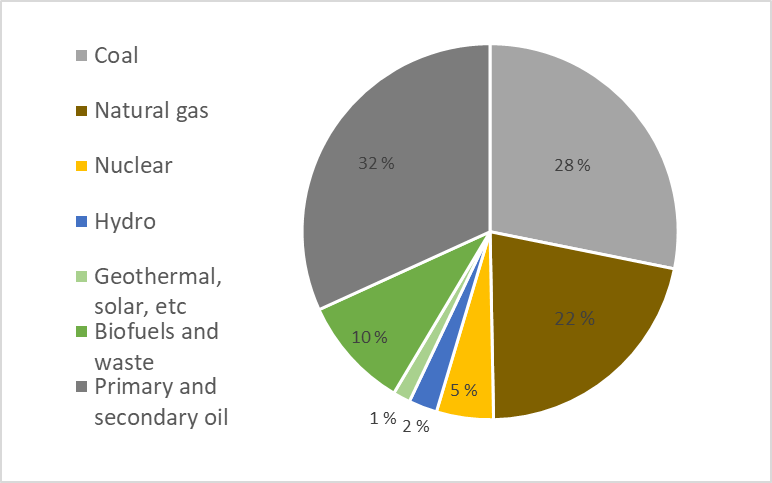
\includegraphics[width=0.45\textwidth]{vedlegg/TPESnew}
    \caption{\textit{Total primary energy supply by source, 2015}}
     \vspace{-6mm}
    \label{fig:TPES}
\end{wrapfigure}

The reason behind this topic is based on global warming, perhaps the greatest challenge the world has ever faced. The global primary energy consumption was in 2015, 13 669 million tonnes of oil equivalent (\ac{Mtoe}), and from figure \ref{fig:TPES}, it can be seen that 81.5\% of that came from the fossil fuels coal, natural gas and oil \cite{stats}. Energy production from fossil fuels results in emissions of the greenhouse gas carbon dioxide (\ac{co2}), and as a consequence of this the concentration of the gas in the atmosphere has increased approximately 1\% yearly from 338.89 ppm in 1980 to 404.97 in 2017 \cite{co2levels}. A graphical representation of CO$_2$ concentration in the atmosphere from 1980 to 2017 is displaced in figure \ref{fig:co2}. 

In the same time period the global average temperature, illustrated in figure \ref{fig:temp}, has increased with 0.63$^\circ$C, and was in 2016 a record high 0.99$^\circ$C above pre-industrial levels \cite{temp}. The global temperature depends on many factors, but a connection between the concentration of CO$_2$ in the atmosphere and the global mean temperature is beyond doubt. As the concentration of CO$_2$ continues to rise, the temperature on the planet is expected to do the same. 

\begin{wrapfigure}{i}{0.5\textwidth}
    \centering
    \vspace{-4mm}
    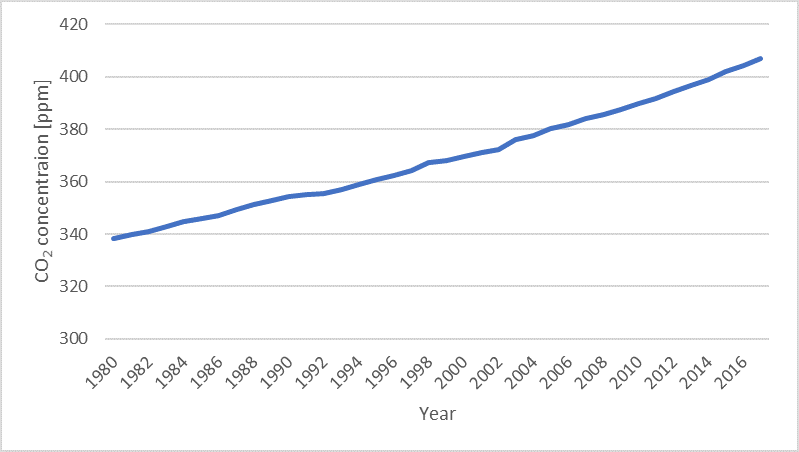
\includegraphics[width=0.4\textwidth]{vedlegg/co2new}
  \caption{\textit{CO$_2$ concentration in the atmosphere from 1980 - 2017}}
  \label{fig:co2}
  \vspace{-30mm}
\end{wrapfigure}


The Paris Agreement on climate change is an agreement signed by more than 190 countries, and a central aim is to reduce the damage of global warming to less than 1.5$^\circ$C rise of global mean temperature compared to pre-industrial levels \cite{paris}. 


\pagebreak

\begin{wrapfigure}{o}{0.4\textwidth}
    \centering
    %\vspace{-4mm}
    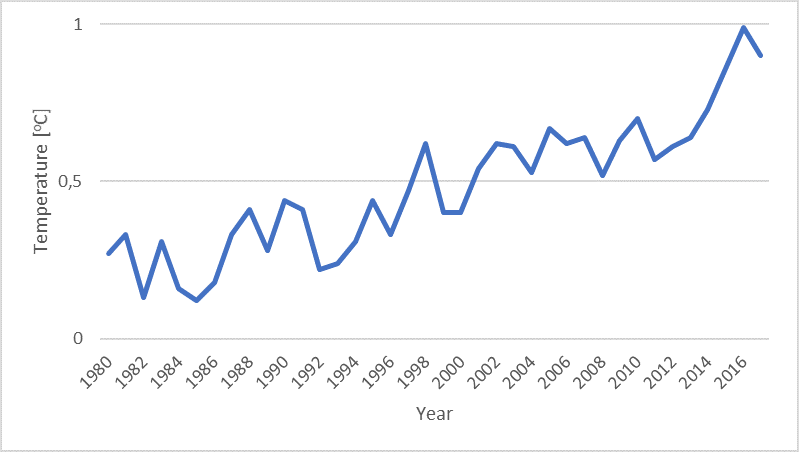
\includegraphics[width=0.4\textwidth]{vedlegg/tempnew}
    \caption{\textit{Global mean temperature from 1980 - 2017, compared to pre-industrial levels}}
    \label{fig:temp}
\end{wrapfigure}

An Intergovernmental Panel on Climate Change (IPCC) special report on the impacts of global warming states that emission of greenhouse gases needs to be reduced by 45\% compared to 2010 by 2030 in order to achieve the goal of the Paris agreement, and there are four main approaches to obtain that goal \cite{Ipcc}. The first and most effective is reducing the energy demand. The second is to replace energy produced by fossil fuels with energy from renewable sources. Solar-, hydro-, wind- and wave energy are examples of energy sources that are renewable. The third approach is to make energy production from fossil fuels more efficient. It is not realistic to cover the  entire global energy demand by renewable sources within 2030, so its important to make use of the energy from fossil fuels most efficient to reduce emissions of greenhouse gases. The last approach is to capture and store greenhouse gases such as CO$_2$ and methane to reduce the levels of the gases in the atmosphere. This report is focusing on the first two approaches as they are most relevant to this topic.

\begin{wrapfigure}{o}{0.5\textwidth}
    \centering
    \vspace{-4mm}
    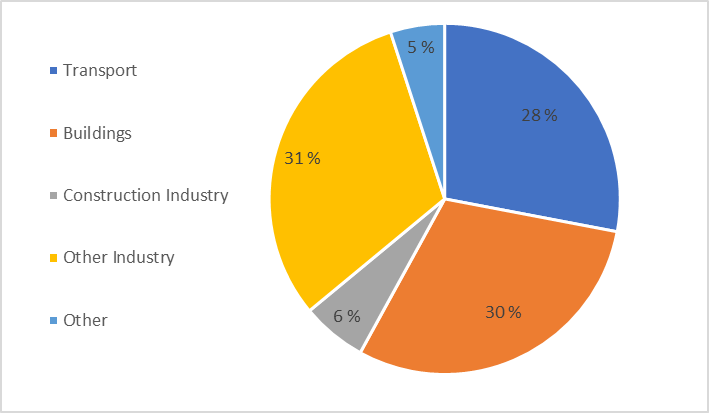
\includegraphics[width=0.5\textwidth]{vedlegg/sec}
    \caption{\textit{Global final energy consumption by sector, 2015}}
    \label{fig:sector}
    \vspace{-4mm}
\end{wrapfigure}

The consequences of a rise in global mean temperature is more extreme weather, drought, floods, rise in sea level because of melting polar ice, which again will lead to areas located at sea level today, under water in the future. The magnitude of this effect all depends on how much the temperature increases, and the difference between 1.5 and 2 or even 3 degrees above pre-industrial levels are severe \cite{Ipcc}. 

The operation of buildings is responsible for 30\% of final energy consumption and more than 55\% of electricity demand globally \cite{ETP}. To accomplish the target of the Paris Agreement, the building sector therefore clearly has a huge responsibility. The energy demand of buildings in the future has to decrease and at the same time produce on site renewable energy.

% - The research question or hypothesis you set out to investigate
This report will analyze the energy consumption of a net Zero Energy Building located in Shanghai, China, with integrated solar thermal and PV systems for cooling, heating, and electricity production. There will be made an economic analysis of the project, and recommendation for further work.
% Towards the end of the introduction, you should also say something about how your text is structured, as a short guide to the reader.

The thesis will first explain the theory behind the technology that is being investigated, before the methodology of the research will be described. Then the development of the model used for energy simulations will be explained and different simulation tools will be discussed. The results of the simulation will then be presented, analyzed and discussed before a conclusion will be drawn. The thesis will end with a plan for further work. 